\documentclass[12pt,letterpaper]{article}\usepackage[]{graphicx}\usepackage[]{color}
%% maxwidth is the original width if it is less than linewidth
%% otherwise use linewidth (to make sure the graphics do not exceed the margin)
\makeatletter
\def\maxwidth{ %
  \ifdim\Gin@nat@width>\linewidth
    \linewidth
  \else
    \Gin@nat@width
  \fi
}
\makeatother

\definecolor{fgcolor}{rgb}{0.345, 0.345, 0.345}
\newcommand{\hlnum}[1]{\textcolor[rgb]{0.686,0.059,0.569}{#1}}%
\newcommand{\hlstr}[1]{\textcolor[rgb]{0.192,0.494,0.8}{#1}}%
\newcommand{\hlcom}[1]{\textcolor[rgb]{0.678,0.584,0.686}{\textit{#1}}}%
\newcommand{\hlopt}[1]{\textcolor[rgb]{0,0,0}{#1}}%
\newcommand{\hlstd}[1]{\textcolor[rgb]{0.345,0.345,0.345}{#1}}%
\newcommand{\hlkwa}[1]{\textcolor[rgb]{0.161,0.373,0.58}{\textbf{#1}}}%
\newcommand{\hlkwb}[1]{\textcolor[rgb]{0.69,0.353,0.396}{#1}}%
\newcommand{\hlkwc}[1]{\textcolor[rgb]{0.333,0.667,0.333}{#1}}%
\newcommand{\hlkwd}[1]{\textcolor[rgb]{0.737,0.353,0.396}{\textbf{#1}}}%

\usepackage{framed}
\makeatletter
\newenvironment{kframe}{%
 \def\at@end@of@kframe{}%
 \ifinner\ifhmode%
  \def\at@end@of@kframe{\end{minipage}}%
  \begin{minipage}{\columnwidth}%
 \fi\fi%
 \def\FrameCommand##1{\hskip\@totalleftmargin \hskip-\fboxsep
 \colorbox{shadecolor}{##1}\hskip-\fboxsep
     % There is no \\@totalrightmargin, so:
     \hskip-\linewidth \hskip-\@totalleftmargin \hskip\columnwidth}%
 \MakeFramed {\advance\hsize-\width
   \@totalleftmargin\z@ \linewidth\hsize
   \@setminipage}}%
 {\par\unskip\endMakeFramed%
 \at@end@of@kframe}
\makeatother

\definecolor{shadecolor}{rgb}{.97, .97, .97}
\definecolor{messagecolor}{rgb}{0, 0, 0}
\definecolor{warningcolor}{rgb}{1, 0, 1}
\definecolor{errorcolor}{rgb}{1, 0, 0}
\newenvironment{knitrout}{}{} % an empty environment to be redefined in TeX

\usepackage{alltt}
 \usepackage[left=2cm,right=2cm,top=2cm,bottom=2cm]{geometry}
\usepackage[ansinew]{inputenc}
\usepackage[spanish]{babel}
\usepackage{amsmath}
\usepackage{amsfonts}
\usepackage{amssymb}
\usepackage{dsfont}
\usepackage{multicol} 
\usepackage{subfigure}
\usepackage{graphicx}
\usepackage{float} 
\usepackage{verbatim} 
\usepackage[left=2cm,right=2cm,top=2cm,bottom=2cm]{geometry}
\usepackage{fancyhdr}
\pagestyle{fancy} 
\fancyhead[LO]{\leftmark}
\usepackage{caption}
\newtheorem{definicion}{Definci\'on}
\IfFileExists{upquote.sty}{\usepackage{upquote}}{}
\begin{document}

\begin{titlepage}
\setlength{\unitlength}{1 cm} %Especificar unidad de trabajo


\begin{center}
\textbf{{\large UNIVERSIDAD DE EL SALVADOR}\\
{\large FACULTAD MULTIDISCIPLINARIA DE OCCIDENTE}\\
{\large DEPARTAMENTO DE MATEM\'ATICA}}\\[0.50 cm]

\begin{picture}(18,4)
 \put(7,0){
\includegraphics[width=4cm]{minerva.jpg}}
\end{picture}
\\[0.25 cm]

\textbf{{\large Licenciatura en Estad\'istica}\\[1.25cm]
{\large Control Estadistico del Paquete R }\\[2 cm]
%\setlength{\unitlength}{1 cm}
{\large  \textbf{''UNIDAD CINCO"}}\\
{\large  \textbf{Pr\'actica 21 - Prueba de hip\'otesis estad\'isticas y prueba de normalidad.}}\\[3 cm]
{\large Alumna:}\\
{\large Martha Yoana Medina S\'anchez}\\[2cm]
{\large Fecha de elaboraci\'on}\\
Santa Ana - \today }
\end{center}
\end{titlepage}

\newtheorem{teorema}{Teorema}
\newtheorem{prop}{Proposici\'on}[section]

\lhead{UNIDAD CINCO}
\chead{PR\'ACTICA 21}
\lfoot{LICENCIATURA EN ESTAD\'ISTICA}
\cfoot{UESOCC}
\rfoot{\thepage}
%\pagestyle{fancy} 

\setcounter{page}{1}
\newpage

\begin{center}
\textbf{1.  FORMULACI\'ON Y PRUEBA DE HIP\'OTESIS}
\end{center}

Los pasos del m\'etodo cient\'ifico se pueden resumir de la siguiente forma:
\begin{enumerate}
  \item Plantear el problema a resolver. 
  \item Efectuar las observaciones.
  \item Formular una o m\'as hip\'otesis. 
  \item Probar dichas hip\'otesis, y
  \item Proclamar las conclusiones.
\end{enumerate}

La Estad\'istica nos puede ayudar en los pasos 2) (dise\~no de las observaciones) y 4) (prueba de hip\'otesis). Una definici\'on de hip\'otesis es la siguiente: "una explicaci\'on tentativa que cuenta con un conjunto de hechos y puede ser probada con una investigaci\'on posterior". La formulaci\'on de una hip\'otesis se logra examinando cuidadosamente las observaciones,para luego proponer un resultado posible.\\

La formulaci\'on formal de una hip\'otesis en el m\'etodo cient\'ifico se realiza definiendo la hip\'otesis nula ($H_0$) y la hip\'otesis alternativa ($H_1$). La hip\'otesis alternativa 
$H_1$, por otra parte, suele indicarse como el complemento de la $H_0$.\\

A la hora de tomar una decisi\'on respecto de la hip\'otesis nula, surgen situaciones que nos pueden llevar a cometer diferentes errores. En los casos que $H_0$ se acepte y sea verdadera, as\'i como tambi\'en en el caso que $H_0$ se rechace y sea falsa, la decisi\'on habr\'a sido la correcta. Pero en los otros dos casos se producen los denominados errores tipo I y tipo II.\\

El error tipo I (o de primera especie), se produce cuando se rechaz\'o $H_0$ y es verdadera,
$alfa$ quien representa la probabilidad de haber cometido este tipo de error y que se conoce como el nivel de significancia, suele fijarse antes de realizar la prueba. En el caso que 
$H_0$ sea aceptada siendo falsa, se cometer\'a el error denominado de tipo II, $beta$ representa la probabilidad de cometer tal error. La potencia de un m\'etodo estad\'istico en una determinada situaci\'on se calcula como ($1-beta$), lo que se corresponde con la situaci\'on de haber rechazado correctamente $H_0$.\\

Una hip\'otesis no se acepta, simplemente la evidencia no alcanza para rechazarla, y se mantiene como cierta mientras no se rechace.\\

En cualquier caso rechazar $H_0$ es lo mismo que aceptar la $H_1$ y viceversa. El resultado final de un m\'etodo estad\'istico para la prueba de una hip\'otesis es el valor p, que indica la probabilidad de obtener un valor m\'as extremo que el observado si $H_0$ es verdadera. Cuando p es menor que $alfa$ se procede a rechazar $H_0$.\\

Por ejemplo, un problema a resolver podr\'ia ser la importancia del estado nutricional en pacientes diab\'eticos con complicaciones; ya tenemos el paso 1) del m\'etodo cient\'ifico; luego efectuamos observaciones en dos grupos de sujetos, uno de control (saludables, denominados de aqu\i en adelante como controles) y otro de diab\'eticos con complicaciones (denominados de aqu\'i en adelante como pacientes); el tama\~no de dichas muestras se basa en estudios similares ya publicados y/o experiencia de los investigadores sobre y/o c\'alculos sobre tama\~no de las muestras.\\

Uno de los indicadores m\'as comunes del estado nutricional de una persona se puede cuantificar con el denominado \'indice de masa corporal (IMC), el cual se define con la siguiente ecuaci\'on:

\begin{center}
$IMC=Peso[Kg]/(Altura[m]^2)   (1)$
\end{center}

Los valores normales (y por lo tanto saludables) del IMC van de 20 a 25 $Kg/m^2$, valores superiores a 25 $Kg/m^2$ y menores de 30 $Kg/m^2$ se consideran como sobrepeso, finalmente IMC iguales o superiores a 30 $Kg/m^2$ se consideran como indicativos de obesidad. Valores altos de IMC son predictores de muerte en algunas patolog\'ias como enfermedades cardiovasculares, diabetes, c\'ancer, hipertensi\'on arterial y osteoartritis. La obesidad por s\'i sola es un factor de riesgo de muerte prematura.\\

Tabla 1: IMC para cada sujeto, Grupo de Control
\begin{knitrout}
\definecolor{shadecolor}{rgb}{0.969, 0.969, 0.969}\color{fgcolor}\begin{kframe}
\begin{alltt}
\hlstd{sujecto} \hlkwb{<-} \hlkwd{c}\hlstd{(}\hlnum{1}\hlstd{,} \hlnum{2}\hlstd{,} \hlnum{3}\hlstd{,} \hlnum{4}\hlstd{,} \hlnum{5}\hlstd{,} \hlnum{6}\hlstd{,} \hlnum{7}\hlstd{,} \hlnum{8}\hlstd{,} \hlnum{9}\hlstd{,} \hlnum{10}\hlstd{,} \hlnum{11}\hlstd{,} \hlnum{12}\hlstd{,} \hlnum{13}\hlstd{,} \hlnum{14}\hlstd{,} \hlnum{15}\hlstd{,} \hlnum{16}\hlstd{,} \hlnum{17}\hlstd{,}
                       \hlnum{18}\hlstd{);}
\hlstd{sujecto}
\end{alltt}
\begin{verbatim}
##  [1]  1  2  3  4  5  6  7  8  9 10 11 12 13 14 15 16 17 18
\end{verbatim}
\begin{alltt}
\hlstd{imc} \hlkwb{<-} \hlkwd{c}\hlstd{(}\hlnum{23.6}\hlstd{,} \hlnum{22.7}\hlstd{,} \hlnum{21.2}\hlstd{,} \hlnum{21.7}\hlstd{,} \hlnum{20.7}\hlstd{,} \hlnum{22.0}\hlstd{,} \hlnum{21.8}\hlstd{,} \hlnum{24.4}\hlstd{,}
                    \hlnum{20.1}\hlstd{,} \hlnum{21.3}\hlstd{,} \hlnum{20.5}\hlstd{,} \hlnum{21.1}\hlstd{,} \hlnum{21.4}\hlstd{,} \hlnum{22.2}\hlstd{,} \hlnum{22.6}\hlstd{,} \hlnum{20.4}\hlstd{,} \hlnum{23.3}\hlstd{,} \hlnum{24.8}\hlstd{);}
\hlstd{imc}
\end{alltt}
\begin{verbatim}
##  [1] 23.6 22.7 21.2 21.7 20.7 22.0 21.8 24.4 20.1 21.3 20.5 21.1 21.4 22.2
## [15] 22.6 20.4 23.3 24.8
\end{verbatim}
\begin{alltt}
\hlstd{hoja1} \hlkwb{<-} \hlkwd{data.frame}\hlstd{(}\hlkwc{Sujecto}\hlstd{=sujecto,} \hlkwc{IMC}\hlstd{=imc); hoja1}
\end{alltt}
\begin{verbatim}
##    Sujecto  IMC
## 1        1 23.6
## 2        2 22.7
## 3        3 21.2
## 4        4 21.7
## 5        5 20.7
## 6        6 22.0
## 7        7 21.8
## 8        8 24.4
## 9        9 20.1
## 10      10 21.3
## 11      11 20.5
## 12      12 21.1
## 13      13 21.4
## 14      14 22.2
## 15      15 22.6
## 16      16 20.4
## 17      17 23.3
## 18      18 24.8
\end{verbatim}
\end{kframe}
\end{knitrout}

Tabla 2: IMC para cada sujeto, Grupo de Pacientes
\begin{knitrout}
\definecolor{shadecolor}{rgb}{0.969, 0.969, 0.969}\color{fgcolor}\begin{kframe}
\begin{alltt}
\hlstd{sujecto} \hlkwb{<-} \hlkwd{c}\hlstd{(}\hlnum{1}\hlstd{,} \hlnum{2}\hlstd{,} \hlnum{3}\hlstd{,} \hlnum{4}\hlstd{,} \hlnum{5}\hlstd{,} \hlnum{6}\hlstd{,} \hlnum{7}\hlstd{,} \hlnum{8}\hlstd{,} \hlnum{9}\hlstd{,} \hlnum{10}\hlstd{,} \hlnum{11}\hlstd{,} \hlnum{12}\hlstd{,} \hlnum{13}\hlstd{,} \hlnum{14}\hlstd{);}
\hlstd{sujecto}
\end{alltt}
\begin{verbatim}
##  [1]  1  2  3  4  5  6  7  8  9 10 11 12 13 14
\end{verbatim}
\begin{alltt}
\hlstd{imc} \hlkwb{<-} \hlkwd{c}\hlstd{(}\hlnum{25.6}\hlstd{,} \hlnum{22.7}\hlstd{,} \hlnum{25.9}\hlstd{,} \hlnum{24.3}\hlstd{,} \hlnum{25.2}\hlstd{,} \hlnum{29.6}\hlstd{,} \hlnum{21.3}\hlstd{,} \hlnum{25.5}\hlstd{,} \hlnum{27.4}\hlstd{,} \hlnum{22.3}\hlstd{,} \hlnum{24.4}\hlstd{,} \hlnum{23.7}\hlstd{,}
         \hlnum{20.6}\hlstd{,} \hlnum{22.8}\hlstd{);}
\hlstd{imc}
\end{alltt}
\begin{verbatim}
##  [1] 25.6 22.7 25.9 24.3 25.2 29.6 21.3 25.5 27.4 22.3 24.4 23.7 20.6 22.8
\end{verbatim}
\begin{alltt}
\hlstd{hoja1} \hlkwb{<-} \hlkwd{data.frame}\hlstd{(}\hlkwc{Sujecto}\hlstd{=sujecto,} \hlkwc{IMC}\hlstd{=imc); hoja1}
\end{alltt}
\begin{verbatim}
##    Sujecto  IMC
## 1        1 25.6
## 2        2 22.7
## 3        3 25.9
## 4        4 24.3
## 5        5 25.2
## 6        6 29.6
## 7        7 21.3
## 8        8 25.5
## 9        9 27.4
## 10      10 22.3
## 11      11 24.4
## 12      12 23.7
## 13      13 20.6
## 14      14 22.8
\end{verbatim}
\end{kframe}
\end{knitrout}

\begin{center}
\textbf{2.  PRUEBAS DE NORMALIDAD DE UNA MUESTRA.}
\end{center}

Antes de proceder a la prueba de una hip\'otesis debemos determinar la distribuci\'on de las variables consideradas en la muestra. En los m\'etodos convencionales se trabaja con la distribuci\'on normal de dichas variables. El paso inicial entonces, es determinar si las variables en estudio pueden ser representadas por una distribuci\'on "normal". En otras palabras necesitamos verificar esta primera hip\'otesis.\\

La importancia de verificar la normalidad de las muestras en estudio es fundamental en estad\'istica porque si las muestras son normales se pueden aplicar m\'etodos estad\'isticos param\'etricos convencionales, en caso contrario se deben o bien transformar los datos, o bien utilizar m\'etodos como los no param\'etricos u otros m\'etodos estad\'isticos m\'as sofisticados.\\

Los m\'etodos de la estad\'istica descriptiva nos pueden ayudar a verificar la normalidad de las variables, un histograma y un gr\'afico de cajas nos muestra en dos formas distintas la distribuci\'on de los datos. Pruebas de normalidad m\'as formales, no param\'etricas, muy recomendables para verificar la normalidad de una variable son las pruebas de Shapiro-Wilk, y de Kolmogorov-Smirnov. Tambi\'en existen los gr\'aficos PP y QQ.\\

Contrariamente a lo que se desea en la mayor\'ia de los casos, en las pruebas de normalidad se busca aceptar $H_0$, dado que en la mayor\'ia de los m\'etodos estad\'isticos convencionales es necesaria la distribuci\'on normal de la variable de inter\'es, siendo posible conocer los par\'ametros que la describen tales como su media ($µ$) y su desviaci\'on est\'andar ($s$) . Un  p - valor mayor a 0.10 en los tests de normalidad indicar\'ia que no hay prueba suficiente para rechazar la normalidad de la variable. Por el contrario un p - valor menor a 0.01 indicar\'ia que nuestros datos no siguen una distribuci\'on normal.\\

A continuaci\'on procedemos a contrastar normalidad para los datos del IMC en los grupos de Control y de Pacientes. Observe que la caracter\'istica de inter\'es debe ser normal en ambos grupos, es decir, la normalidad se estudia en cada uno de ellos y noen la informaci\'on combinada de los grupos.\\

El siguiente c\'odigo en lenguaje R podr\'ia ser utilizado para dichos fines:
\begin{knitrout}
\definecolor{shadecolor}{rgb}{0.969, 0.969, 0.969}\color{fgcolor}\begin{kframe}
\begin{alltt}
\hlcom{#se digitan los datos del grupo de control}

\hlstd{IMC_Control}\hlkwb{<-}\hlkwd{c}\hlstd{(}\hlnum{23.6}\hlstd{,} \hlnum{22.7}\hlstd{,} \hlnum{21.2}\hlstd{,} \hlnum{21.7}\hlstd{,} \hlnum{20.7}\hlstd{,} \hlnum{22.0}\hlstd{,} \hlnum{21.8}\hlstd{,} \hlnum{24.2}\hlstd{,} \hlnum{20.1}\hlstd{,} \hlnum{21.3}\hlstd{,} \hlnum{20.5}\hlstd{,}
                 \hlnum{21.1}\hlstd{,} \hlnum{21.4}\hlstd{,} \hlnum{22.2}\hlstd{,} \hlnum{22.6}\hlstd{,} \hlnum{20.4}\hlstd{,} \hlnum{23.3}\hlstd{,} \hlnum{24.8}\hlstd{)}
\hlkwd{par}\hlstd{(}\hlkwc{mfrow}\hlstd{=}\hlkwd{c}\hlstd{(}\hlnum{1}\hlstd{,}\hlnum{2}\hlstd{))}

\hlcom{#se genera el histograma de la variables de inter\textbackslash{}'es }

\hlkwd{hist}\hlstd{(IMC_Control,}\hlkwc{main}\hlstd{=}\hlstr{"A"}\hlstd{,}\hlkwc{xlab}\hlstd{=}\hlstr{"IMC (kg/m2)"}\hlstd{,}\hlkwc{ylab}\hlstd{=}\hlstr{"Frecuencia"}\hlstd{,}\hlkwc{col}\hlstd{=}\hlstr{"blue"}\hlstd{)}

\hlcom{# se genera el diagrama de caja de la variable de inter\textbackslash{}'es y se muestra en }
\hlcom{# la misma ventana }

\hlkwd{boxplot}\hlstd{(IMC_Control,}\hlkwc{main}\hlstd{=}\hlstr{"B"}\hlstd{,} \hlkwc{lab}\hlstd{=}\hlstr{"IMC (kg/m2)"}\hlstd{,}\hlkwc{ylim}\hlstd{=}\hlkwd{c}\hlstd{(}\hlnum{20}\hlstd{,}\hlnum{25}\hlstd{),} \hlkwc{col}\hlstd{=}\hlstr{"green"}\hlstd{)}
\end{alltt}
\end{kframe}
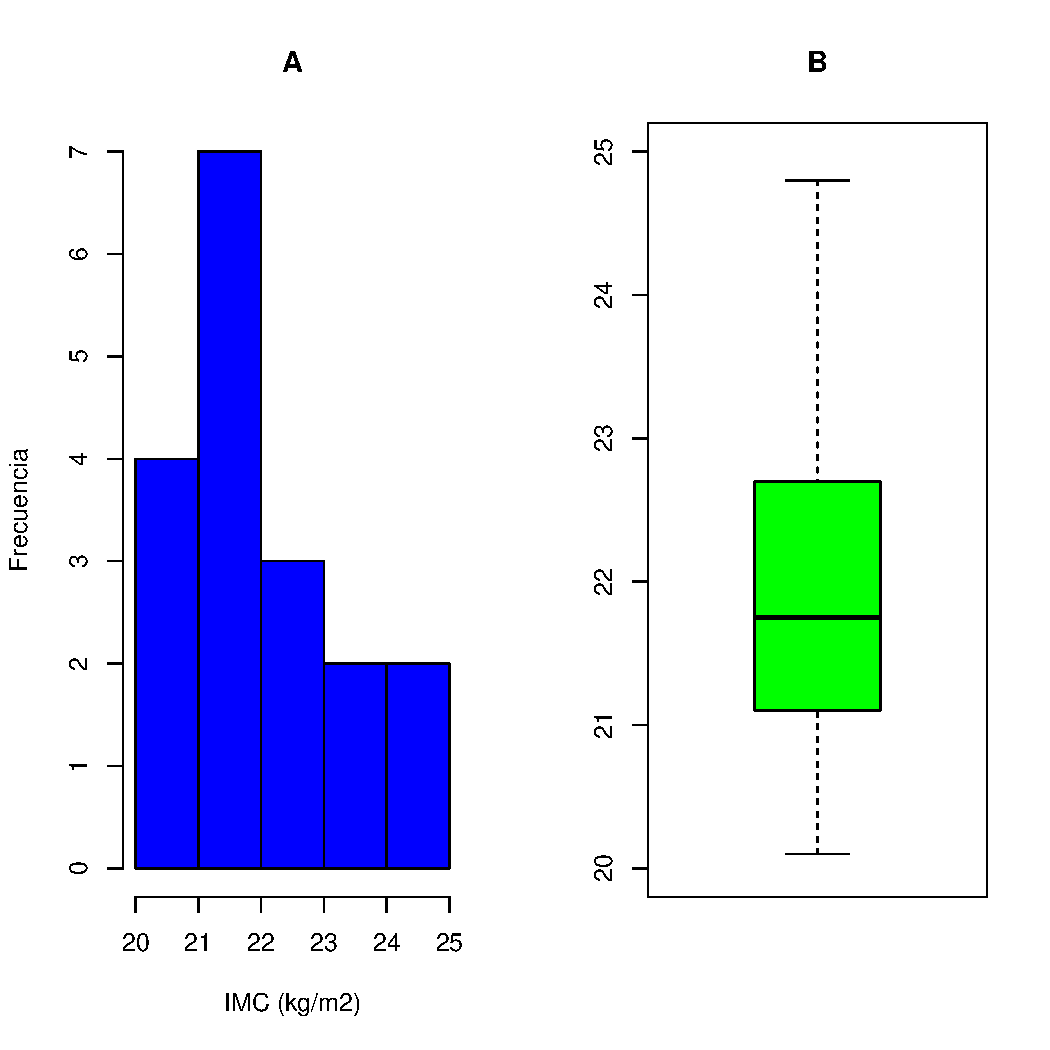
\includegraphics[width=\maxwidth]{figure/unnamed-chunk-3-1} 
\begin{kframe}\begin{alltt}
\hlcom{# los commandos para contrastar normalidad son los siguientes }

\hlstd{sw} \hlkwb{<-} \hlkwd{shapiro.test}\hlstd{(IMC_Control)}
\hlstd{sw}
\end{alltt}
\begin{verbatim}
## 
## 	Shapiro-Wilk normality test
## 
## data:  IMC_Control
## W = 0.95321, p-value = 0.4776
\end{verbatim}
\begin{alltt}
\hlcom{# note que en la prueba de Shapiro solo es necesario especificar la variable que }
\hlcom{# se est\textbackslash{}'a contrastado. ESTA PRUEBA SOLAMENTE SEUTILIZA PARA VERIFICAR NORMALIDAD. }

\hlstd{ks} \hlkwb{<-} \hlkwd{ks.test}\hlstd{(IMC_Control,}\hlstr{"pnorm"}\hlstd{,}\hlkwc{mean}\hlstd{=}\hlkwd{mean}\hlstd{(IMC_Control),}\hlkwc{sd}\hlstd{=}\hlkwd{sd}\hlstd{(IMC_Control))}
\hlstd{ks}
\end{alltt}
\begin{verbatim}
## 
## 	One-sample Kolmogorov-Smirnov test
## 
## data:  IMC_Control
## D = 0.11172, p-value = 0.9595
## alternative hypothesis: two-sided
\end{verbatim}
\begin{alltt}
\hlcom{# note que la prueba de Kolmogorov es m\textbackslash{}'as general, permite contrastar cualquier }
\hlcom{# tipo de distribuci\textbackslash{}'on, en "pnorm" se indicaque la distribuci\textbackslash{}'on que se desea }
\hlcom{# contrastar es la normal; sin embargo, es necesario especificar los par\textbackslash{}'ametros }
\hlcom{# de la distribuci\textbackslash{}'on media (mean) y desviaci\textbackslash{}'on (sd) estimados a partir de los }
\hlcom{# datos.}

\hlcom{# Luego se digitan los datos para pacientes y se ejecutan las mismas instrucciones }

\hlstd{IMC_Pacientes} \hlkwb{<-} \hlkwd{c}\hlstd{(}\hlnum{25.6}\hlstd{,} \hlnum{22.7}\hlstd{,} \hlnum{25.9}\hlstd{,} \hlnum{24.3}\hlstd{,} \hlnum{25.2}\hlstd{,} \hlnum{29.6}\hlstd{,} \hlnum{21.3}\hlstd{,} \hlnum{25.5}\hlstd{,} \hlnum{27.4}\hlstd{,} \hlnum{22.3}\hlstd{,} \hlnum{24.4}\hlstd{,}
                   \hlnum{23.7}\hlstd{,} \hlnum{20.6}\hlstd{,} \hlnum{22.8}\hlstd{)}
\end{alltt}
\end{kframe}
\end{knitrout}

\begin{knitrout}
\definecolor{shadecolor}{rgb}{0.969, 0.969, 0.969}\color{fgcolor}\begin{kframe}
\begin{alltt}
\hlstd{IMC_Pacientes} \hlkwb{<-} \hlkwd{c}\hlstd{(}\hlnum{25.6}\hlstd{,} \hlnum{22.7}\hlstd{,} \hlnum{25.9}\hlstd{,} \hlnum{24.3}\hlstd{,} \hlnum{25.2}\hlstd{,} \hlnum{29.6}\hlstd{,} \hlnum{21.3}\hlstd{,} \hlnum{25.5}\hlstd{,} \hlnum{27.4}\hlstd{,} \hlnum{22.3}\hlstd{,} \hlnum{24.4}\hlstd{,}
                   \hlnum{23.7}\hlstd{,} \hlnum{20.6}\hlstd{,} \hlnum{22.8}\hlstd{)}
\hlkwd{par}\hlstd{(}\hlkwc{mfrow}\hlstd{=}\hlkwd{c}\hlstd{(}\hlnum{1}\hlstd{,}\hlnum{2}\hlstd{))}

\hlcom{#se genera el histograma de la variables de inter\textbackslash{}'es }

\hlkwd{hist}\hlstd{(IMC_Control,}\hlkwc{main}\hlstd{=}\hlstr{"A"}\hlstd{,}\hlkwc{xlab}\hlstd{=}\hlstr{"IMC (kg/m2)"}\hlstd{,}\hlkwc{ylab}\hlstd{=}\hlstr{"Frecuencia"}\hlstd{,}\hlkwc{col}\hlstd{=}\hlstr{"blue"}\hlstd{)}

\hlcom{# se genera el diagrama de caja de la variable de inter\textbackslash{}'es y se muestra en }
\hlcom{# la misma ventana }

\hlkwd{boxplot}\hlstd{(IMC_Pacientes,}\hlkwc{main}\hlstd{=}\hlstr{"B"}\hlstd{,} \hlkwc{lab}\hlstd{=}\hlstr{"IMC (kg/m2)"}\hlstd{,}\hlkwc{ylim}\hlstd{=}\hlkwd{c}\hlstd{(}\hlnum{20}\hlstd{,}\hlnum{25}\hlstd{),} \hlkwc{col}\hlstd{=}\hlstr{"green"}\hlstd{)}
\end{alltt}
\end{kframe}
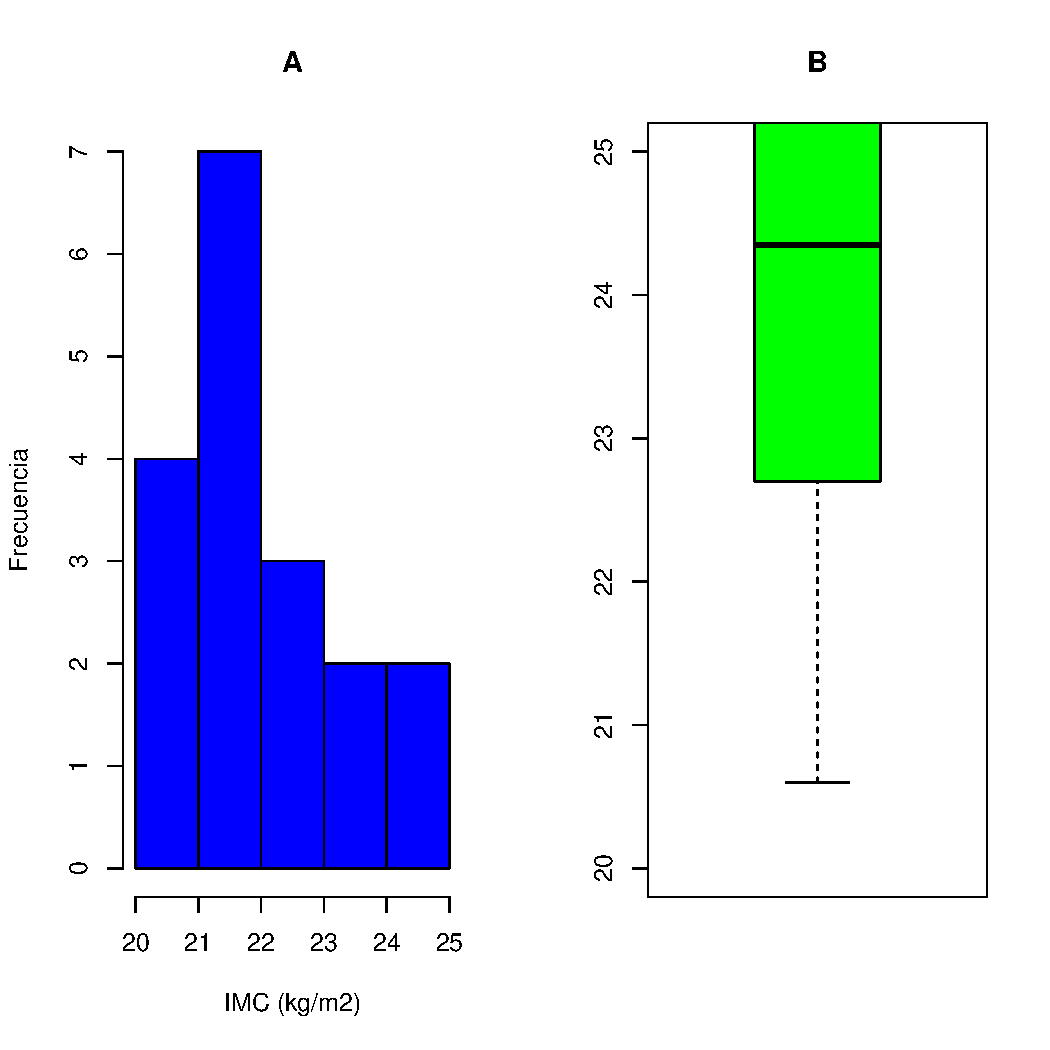
\includegraphics[width=\maxwidth]{figure/unnamed-chunk-4-1} 
\begin{kframe}\begin{alltt}
\hlcom{# los commandos para contrastar normalidad son los siguientes }

\hlstd{sw} \hlkwb{<-} \hlkwd{shapiro.test}\hlstd{(IMC_Pacientes)}
\hlstd{sw}
\end{alltt}
\begin{verbatim}
## 
## 	Shapiro-Wilk normality test
## 
## data:  IMC_Pacientes
## W = 0.97437, p-value = 0.929
\end{verbatim}
\begin{alltt}
\hlcom{# note que en la prueba de Shapiro solo es necesario especificar la variable que }
\hlcom{# se est\textbackslash{}'a contrastado. ESTA PRUEBA SOLAMENTE SEUTILIZA PARA VERIFICAR NORMALIDAD. }

\hlstd{ks} \hlkwb{<-} \hlkwd{ks.test}\hlstd{(IMC_Pacientes,}\hlstr{"pnorm"}\hlstd{,}\hlkwc{mean}\hlstd{=}\hlkwd{mean}\hlstd{(IMC_Pacientes),}\hlkwc{sd}\hlstd{=}\hlkwd{sd}\hlstd{(IMC_Pacientes))}
\hlstd{ks}
\end{alltt}
\begin{verbatim}
## 
## 	One-sample Kolmogorov-Smirnov test
## 
## data:  IMC_Pacientes
## D = 0.12172, p-value = 0.9695
## alternative hypothesis: two-sided
\end{verbatim}
\begin{alltt}
\hlcom{# note que la prueba de Kolmogorov es m\textbackslash{}'as general, permite contrastar cualquier }
\hlcom{# tipo de distribuci\textbackslash{}'on, en "pnorm" se indicaque la distribuci\textbackslash{}'on que se desea }
\hlcom{# contrastar es la normal; sin embargo, es necesario especificar los par\textbackslash{}'ametros }
\hlcom{# de la distribuci\textbackslash{}'on media (mean) y desviaci\textbackslash{}'on (sd) estimados a partir de los }
\hlcom{# datos.}
\end{alltt}
\end{kframe}
\end{knitrout}

\begin{center}
\textbf{3.  PRUEBAS SOBRE MUESTRAS NO NORMALES.}
\end{center}

Hasta el momento en el ejemplo anterior la distribuci\'on de los datos es normal, por lo cual la aplicaci\'on de pruebas param\'etricas normales es totalmente v\'alido. \¿Qu\'e pasa si estamos ante muestras no normales? la respuesta obvia es que nos olvidamos de las pruebas param\'etricas y buscamos la equivalente no param\'etrica, pero siempre que se pueda es aconsejable transformar la muestra para que tenga distribuci\'on normal y as\'i poder aplicar los m\'etodos cl\'asicos.\\

La transformaci\'on de la cual estamos hablando es num\'erica, puede ser simplemente calcular el logaritmo natural de cada observaci\'on, y luego verificar la normalidad de la muestra transformada.\\

Por lo tanto el test medir\'a si los $logaritmos$ de las variables difieren o no, en este caso se deber\'ia considerar si esto tiene interpretaci\'on biol\'ogica.\\

Un comentario especial merecen las pruebas de normalidad, a veces omitidas por algunos 
investigadores, pero que se consideran como fundamentales para poder verificar la normalidad de las muestras, y de esta forma poder aplicar apropiadamente las pruebas estad\'isticas param\'etricas. La prueba de normalidad de Shapiro-Wilk est\'a considerada como la m\'as poderosa para verificar la normalidad de una muestra, por lo cual algunos estad\'isticos consideran que por s\'i sola es suficiente.\\












\end{document}
